\section{Clonal Selection Algorithm}

\begin{frame}
\centering
\Huge \textbf{Clonal Selection Algorithm} 
\\
\large \rightline {Cao,Jing \quad}
\end{frame}

\begin{frame}{The Clonal Selection Theory}
\begin{itemize}
\item{1. B cell products antibodies(Ab) when an animal is exposed to an antigen;}
\item{2. Each B cell secrets only one kind of antibody, which is relatively specific for antigen;}
\item{3. The antigen stimulates the B cell to proliferate(divide) and mature into terminal (non-dividing) antibody secreting cells, called plasma cells;}
\end{itemize}
\end{frame}


\begin{frame}{The Clonal Selection Theory}
\begin{columns}[c] 
\column{.45\textwidth} 
\begin{itemize}
\item{4. Lymphocytes, in addition to proliferating and/or differentiating into plasma cells, can differentiate into long-lived B  memory cells;}
\item{5. When exposed to the same antigen again, the B memory cells can differentiate into large lymphocytes quickly to produce high affinity antibodies;}
\end{itemize}
\column{.55\textwidth} 
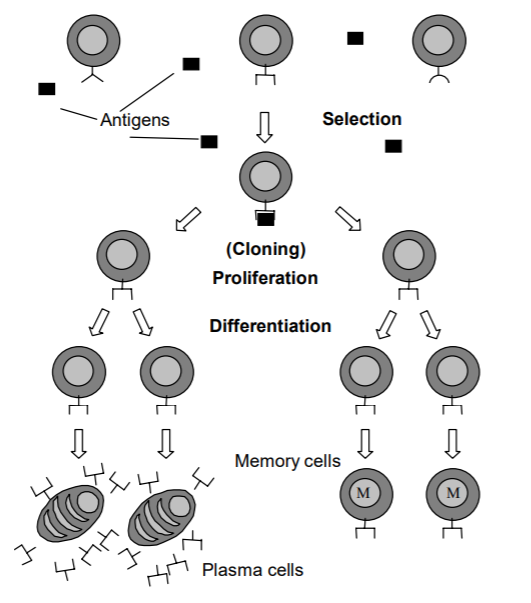
\includegraphics[height=6cm]{img/cj_clone_selection_p.png}
\end{columns}
\end{frame}

\begin{frame}{Reinforcement Learning and Memory}
\begin{columns}[c] 
\column{.45\textwidth}
\begin{itemize}
\item{1. The effectiveness of the immune response to secondary encounters is considerably enhanced  \textcolor{red}{by storing some high affinity antibody} producing cells from the first infection;}
\item{2. Such a strategy ensures that both the speed and accuracy of the immune response \textcolor{red}{becomes successively greater after each infection};}
\item{This scheme is intrinsic of a \textcolor{red}{reinforcement learning strategy} }
\end{itemize}
\column{.55\textwidth} 
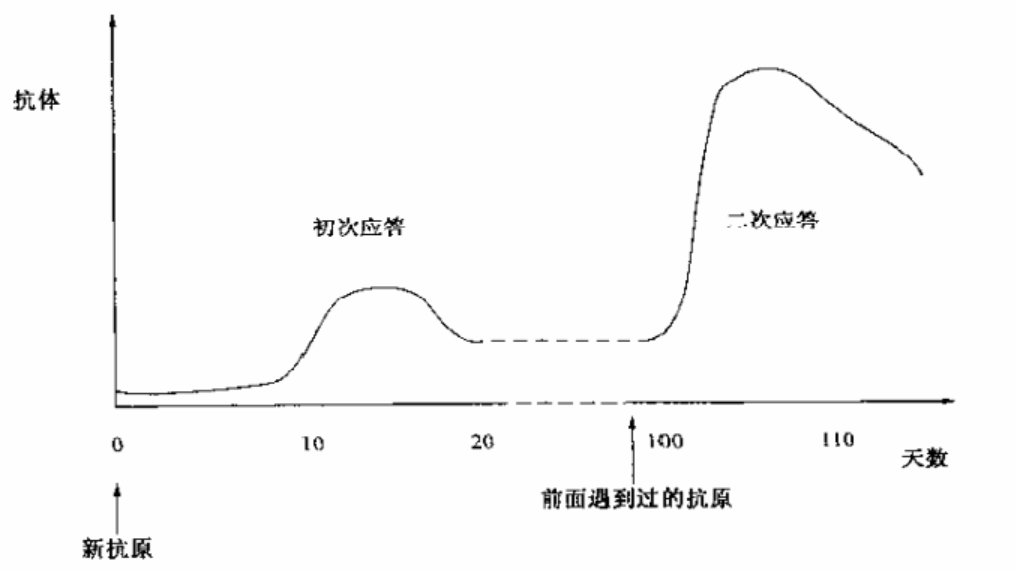
\includegraphics[height=4cm]{img/cj_reinfor_learn.png}
\end{columns}
\end{frame}


\begin{frame}{Reinforcement Learning and Memory}
\begin{itemize}
\item{One important characteristic of the immune memory is that it is associative: B cells adapted to a certain type of antigen A1 presents a faster and more efficient secondary response not only to A1, \textcolor{red}{but also to any structurally related antigen A2.  This phenomenon is called immunological cross-reaction, or cross-reactive response}.}
\item{Antibodies present in a memory response have, \textcolor{red}{on average, a higher affinity than those of the early primary response}. This phenomenon, is referred to as the maturation of the immune response}
\end{itemize}
\end{frame}


\begin{frame}{Somatic Hypermutation, Receptor Editing and Repertoire Diversity}
\begin{columns}[c] 
\column{.45\textwidth} 
\begin{itemize}
\item{1. Point mutations allow the immune system to explore local areas around A by making \textcolor{red}{small steps} towards an antibody with higher affinity;}
\item{2. Receptor editing allows an antibody to take \textcolor{red}{large steps} through the landscape, landing in a locale where the affinity might be lower;}
\end{itemize}
\column{.55\textwidth} 
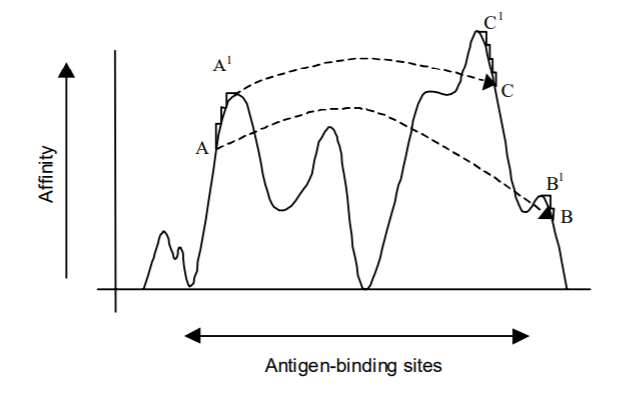
\includegraphics[height=4.5cm]{img/cj_somatic_muta.png}
\end{columns}
\end{frame}

\begin{frame}{The Regulation of the Hypermutation Mechanism}
\begin{itemize}
\item{1. The majority of the mutations  will lead to poorer or non-functional antibodies;}
\item{2. If a cell mutate at a fixed rate, the accumulation of deleterious changes may cause the loss of the advantageous mutation;}
\item{\textcolor{red}{So there should be a selection mechanism}}
\end{itemize}
\end{frame}


\begin{frame}{The Regulation of the Hypermutation Mechanism}
\begin{itemize}
\item{Cells with low affinity receptors may be further mutated and, as a rule, \textcolor{red}{die} if they do not become higher affinity cells. In cells with high-affinity antibody receptors however, hypermutation may be \textcolor{red}{inactivated}.}
\end{itemize}
\end{frame}

\begin{frame}{The Shape-Space Model}
\begin{itemize}
\item{1. The shape-space model (\begin{math} S\end{math}) aims at quantitatively describing the interactions among antigens and antibodies (be \textcolor{red}{Ag-Ab});}
\item{2. The set of features that characterize a molecule is called its \textcolor{red}{generalized shape};}
\item{
3. Mathematically, the generalized shape of a molecule (\begin{math} m\end{math}), either an antibody or an antigen, can be represented by a set of coordinates \begin{math} m =\left \langle m_1, m_2,..., m_L\right\rangle\end{math}, which can be regarded as a point in an \\
L-dimensional real-valued shape-space (m \in S^L);
}
\end{itemize}
\end{frame}



\begin{frame}{The Proposed Algorithm}
\begin{columns}[c] 
\column{.45\textwidth} 
\begin{itemize}
\item{After each six steps we have one cell generation}
\item{(1) Generate a set of (\begin{math} P \end{math}) of candidate solutions, composed of the subset of memory cells  (\begin{math} M \end{math}) added to the remaining (\begin{math} P_r \end{math}) population (\begin{math} P = P_r + M \end{math});}
\item{(2) Determine (Select) the n best individuals of population (\begin{math} P_n \end{math}), based on affinity measure;}
\end{itemize}
\column{.55\textwidth} 
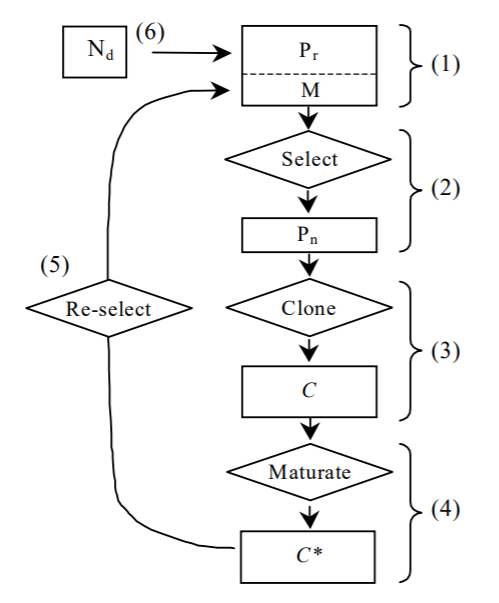
\includegraphics[height=6.5cm]{img/cj_block_diagram_CSA.png}
\end{columns}
\end{frame}


\begin{frame}{The Proposed Algorithm}
\begin{columns}[c] 
\column{.45\textwidth} 
\begin{itemize}
\item{(3) Reproduce (Clone) these n best individuals of the population, giving rise to a temporary population of clones (\begin{math} C \end{math}). The clone size is an increasing function of the affinity with the antigen;}
\item{(4) Submit the population of clones to a hypermutation scheme, where the hypermutation is proportional to the affinity of the antibody with the antigen. A maturated antibody population is generated (\begin{math} C^* \end{math});}
\end{itemize}
\column{.55\textwidth} 
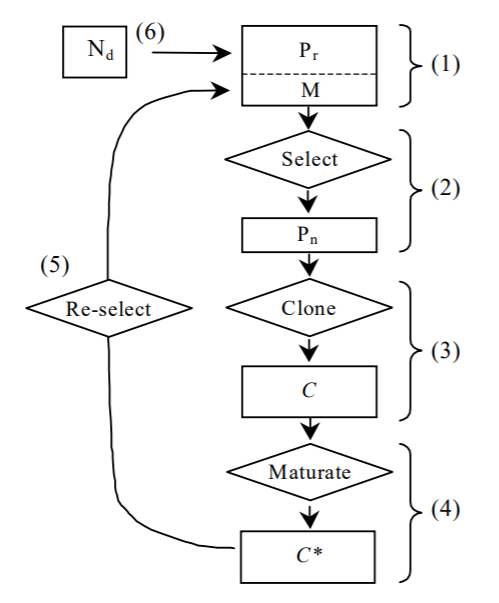
\includegraphics[height=6.5cm]{img/cj_block_diagram_CSA.png}
\end{columns}
\end{frame}


\begin{frame}{The Proposed Algorithm}
\begin{columns}[c] 
\column{.45\textwidth} 
\begin{itemize}
\item{(5) Re-select the improved individuals from \begin{math} C^* \end{math} to compose the memory set \begin{math} M \end{math}. Some members of \begin{math} P \end{math} can be replaced by other improved members of \begin{math} C^* \end{math};}
\item{(6) Replace \begin{math} d \end{math} antibodies by novel ones (diversity introduction). The lower affinity cells have higher probabilities of being replaced;}
\end{itemize}
\column{.55\textwidth} 
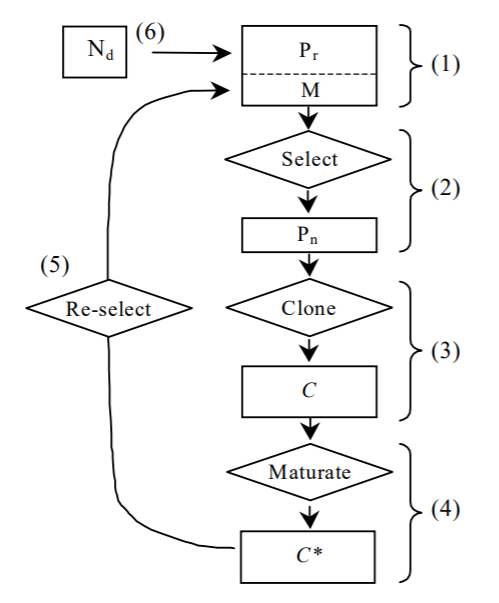
\includegraphics[height=6.5cm]{img/cj_block_diagram_CSA.png}
\end{columns}
\end{frame}

\begin{frame}{Engineering Applications}{Binary Character Recognition}
\begin{itemize}
\item{The goal is to demonstrate that a cumulative blind variation together with selection can \textcolor{red}{produce individuals with increasing affinities} (maturation of the immune response);}
\item{In this case, we assume that the antigen population is represented by a set of eight binary characters to be learned. ;}
\item{Each character is represented by a bitstring of length \begin{math} L = 120 \end{math};}
\end{itemize}

\includegraphics[height=1.5cm]{img/cj_bitsstring.png}
\end{frame}


\begin{frame}{Engineering Applications}{Binary Character Recognition}
\begin{itemize}
\item{The affinity measure takes into account the Hamming distance (\begin{math} D \end{math}) between antigens and antibodies, according to Equation (1):}
\begin{equation} \small{
 D =\sum_{i=1}^{L} \delta \quad where \  \delta = \begin{cases} 1 & \mbox{ if } \  ab_i \neq ag_i \\
 0  & otherwise \end{cases}}
 \end{equation}
\end{itemize}
\end{frame}

\begin{frame}{Engineering Applications}{Binary Character Recognition}
\begin{figure}[h]
\centering
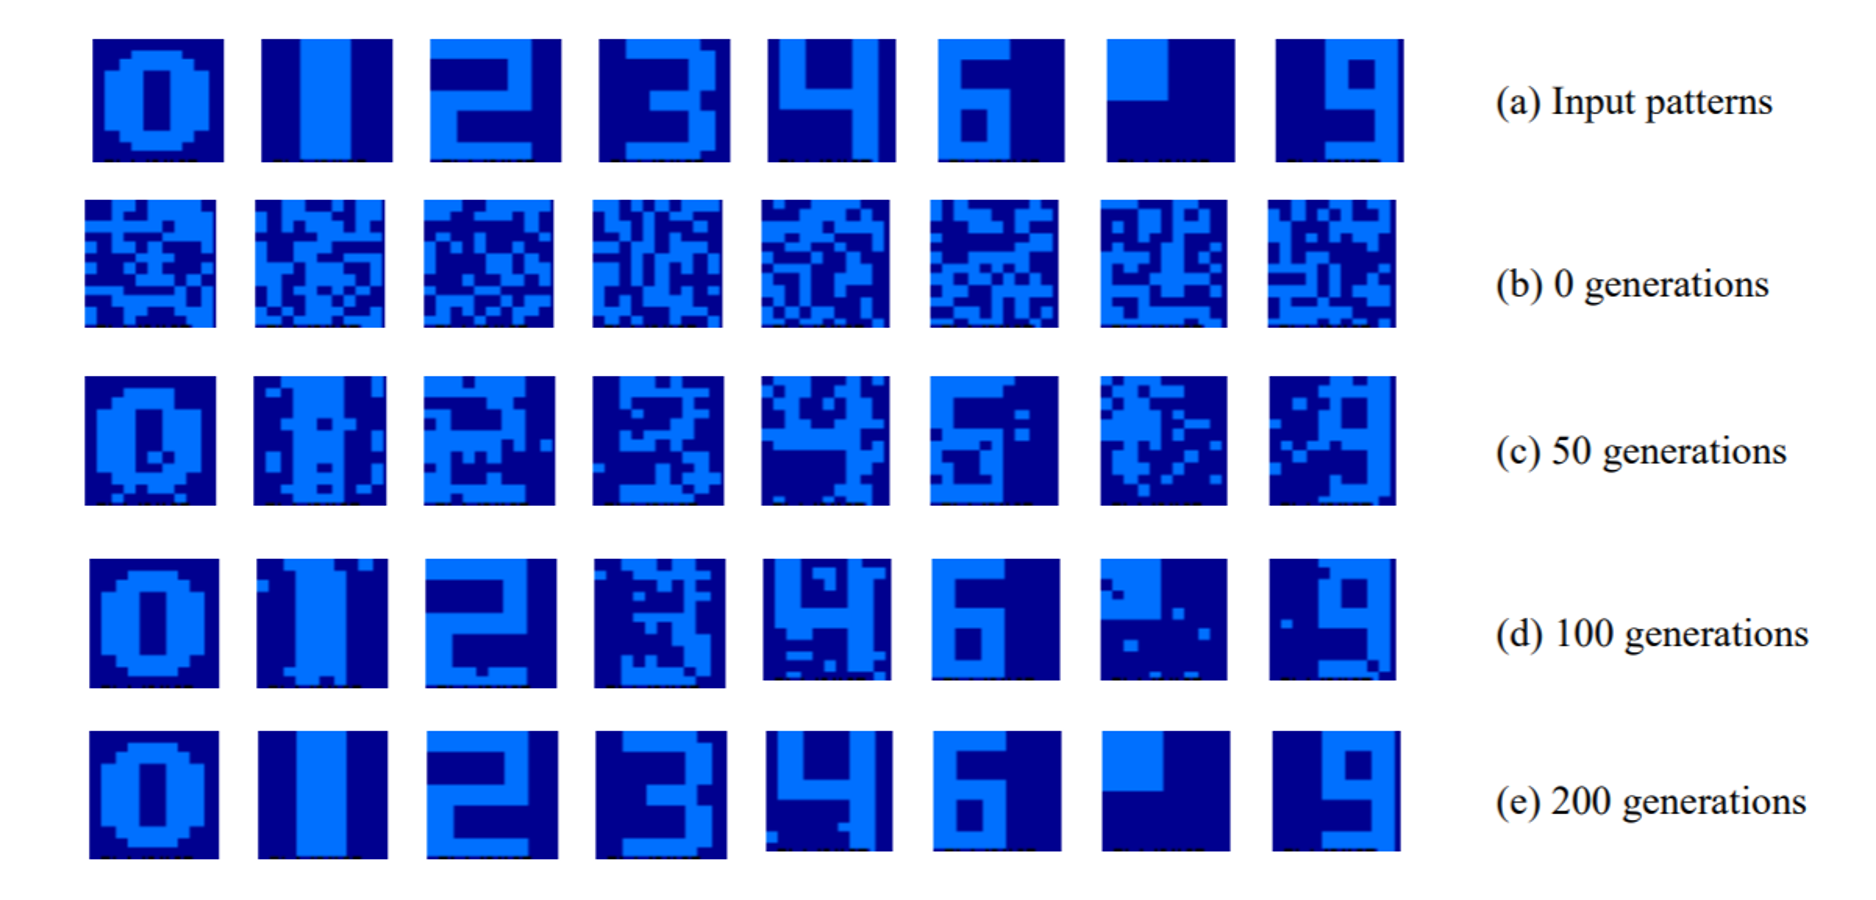
\includegraphics[height=6cm]{img/cj_binary_pattern_learn.png}
\end{figure}
\end{frame}


\begin{frame}{Engineering Applications}{Multi-Modal Optimization}
\begin{itemize}
\item{The CSA reproduces those individuals with higher affinities and selects their improved maturated progenies;} 
\item{This strategy suggests that the algorithm performs a greedy search, where single members will be locally optimized (exploitation of the surrounding space), and the newcomers yield a broader exploration of the searchspace;}
\item{This characteristic makes the CSA \textcolor{red}{very suitable for solving multi-modal optimization tasks}}
\end{itemize}
\end{frame}

\begin{frame}{Engineering Applications}{Multi-Modal Optimization}
\begin{itemize}
\item{Consider the maximizing the function:}
\begin{equation} \small{
f(x, y) = x \cdot sin(4 \pi x) - y \cdot sin(4 \pi y + \pi) +1}
 \end{equation}
\end{itemize}
\begin{figure}[h]
\centering
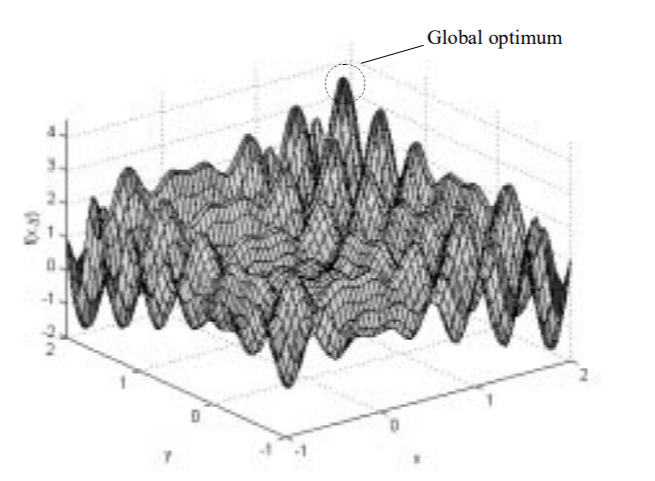
\includegraphics[height=5.5cm]{img/cj_func_maxi.png}
\end{figure}
\end{frame}


\begin{frame}{Engineering Applications}{Multi-Modal Optimization}
\begin{itemize}
\item{We employed the Hamming shape-space, with binary strings representing real values for \begin{math} x \end{math} and \begin{math} y \end{math};}
\item{The chosen bitstring length was \begin{math} L = 22 \end{math},  corresponding to a precision of six decimal places}
\item{The variables \begin{math} x \end{math} and \begin{math} y \end{math} are defined over the range \begin{math} [-1, 2]\end{math},  and the mapping from a binary string  \begin{math} m =\left \langle m_L,..., m_2, m_1\right\rangle\end{math} into a real number \begin{math} z \end{math} is completed in two steps:}
\begin{itemize}
    \item {convert the binary string \begin{math} m =\left \langle m_L,..., m_2, m_1\right\rangle\end{math} from base 2 to base 10:}
    \begin{equation}\small{(<m_L,..., m_2, m_1>)_2 = (\sum_{i=0}^{21}m_i \cdot 2^i)_{10} \ = \ z^{'}}
    \end{equation}
    \item{find the corresponding real value for \begin{math} z \end{math}:}
    \begin{equation}\small{z=z_{min} + z^{'} \cdot \frac{z_{max} - z_{min}}{2^{22} - 1}, \ where \ z_{max} = 2 \ and \ z_{min} = -1
    }
    \end{equation}
\end{itemize}
\end{itemize}
\end{frame}


\begin{frame}{Engineering Applications}{Multi-Modal Optimization}
\begin{itemize}
\item{The affinity measure corresponds to the evaluation of the
function \begin{math} f(x, y) \end{math} after decoding \begin{math} x \end{math} and \begin{math} y \end{math}, as described above;}
\item{The figure below present the  optimized population after 100
generations:}
\end{itemize}
\begin{figure}[h]
\centering
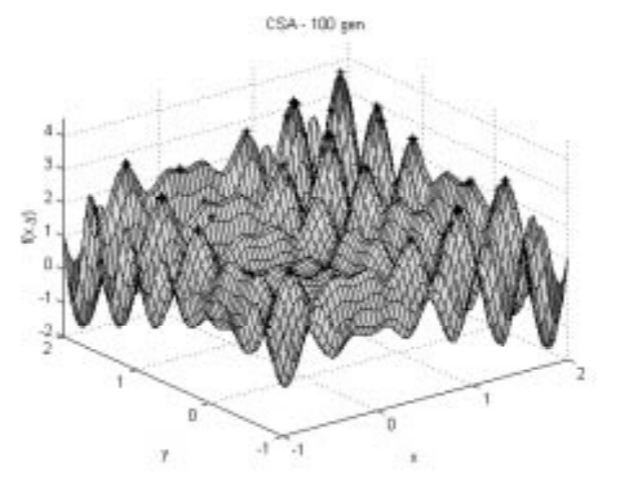
\includegraphics[height=5.5cm]{img/cj_func_maxi_100.png}
\end{figure}
\end{frame}

\begin{frame}{Engineering Applications}{Multi-Modal Optimization}
\begin{itemize}
\item{Notice that the solutions (stars) covers most of the peaks, including the global optimum. }
\end{itemize}
\begin{figure}[h]
\centering
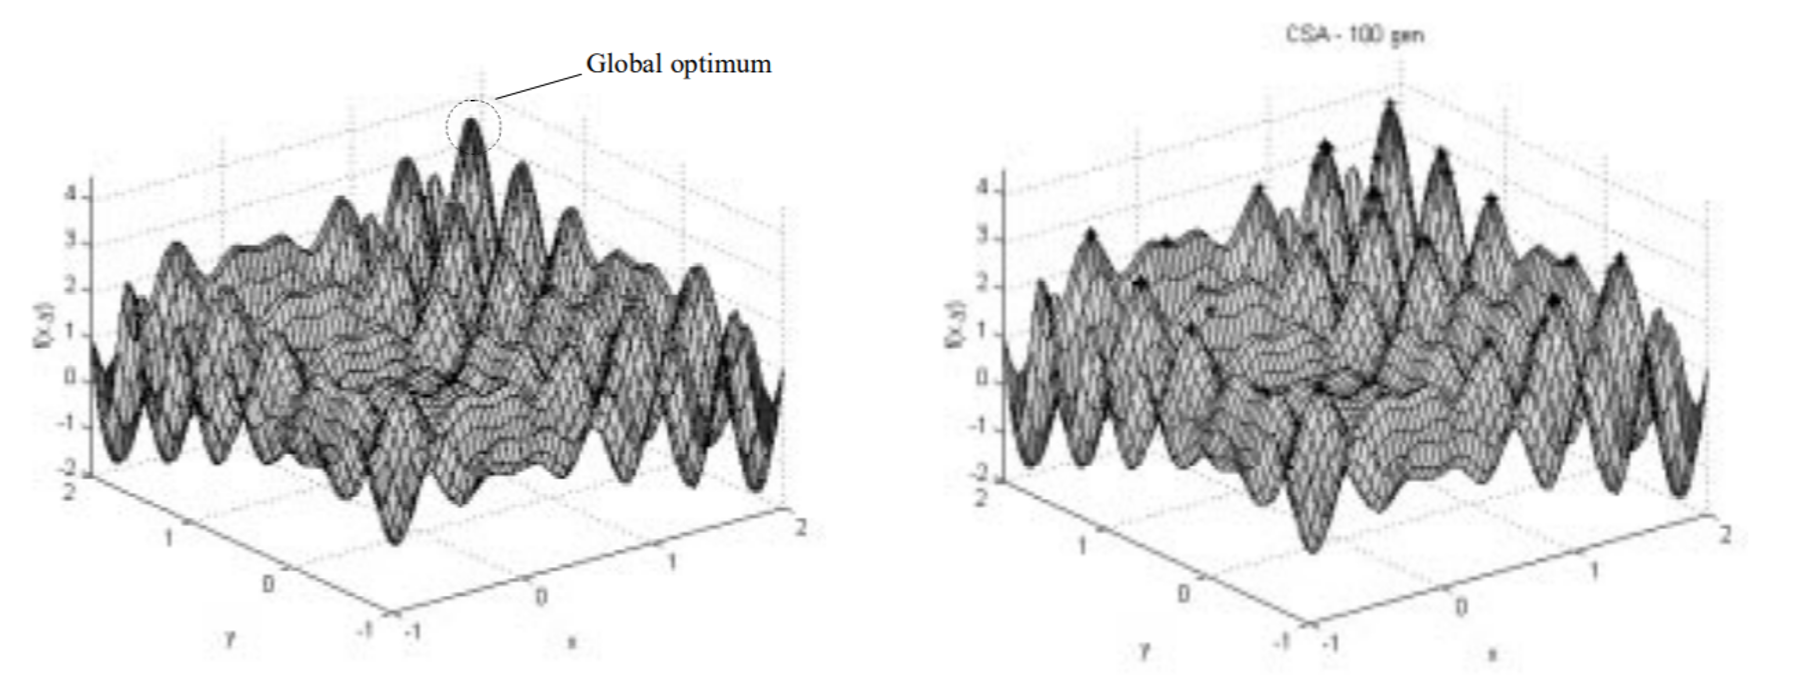
\includegraphics[height=4.5cm]{img/cj_func_and.png}
\end{figure}
\end{frame}


\begin{frame}{Conclusion}
\begin{itemize}
\item{The algorithm was verified to be capable of performing learning and maintenance of high quality memory and, it was also capable of solving complex problems, like multi-modal and combinatorial optimization.}
\end{itemize}

\end{frame}

%  D=\left \{\left \langle s,T_d\right \rangle | s \in P , T_d \in N \right \}}